\section{Projektplan}
\subsection{Teoretisk bakgrund}
När ett tåg ska svänga finns det flera aspekter som måste tas hänsyn till, där kurvradien och hastigheten är två av dem. Om denna radie är för liten eller om tågets hastighet är för hög kommer tåget vältas. Detta eftersom centrifugalkraften flyttar tyngdpunkten så den överskrider rotationsaxeln.
\subsection{Syfte}
Beskriv här syftet, alltså varför ni vill göra just i den här undersökningen, vad ni vill uppnå med resultaten eller hur resultaten kan bidra till förståelsen av det generella problem ni skrivit om i den teoretiska bakgrunden. Här skriver ni vad ni vill uppnå med ert gymnasiearbete. Ni kan till exempel börja med: Syftet med vårt gymnasiearbete är att beskriva/förklara/utvärdera/förstå … Beskriv också här kort hur ni planerar att uppnå syftet med arbetet. Ni kan till exempel skriva: I det här arbetet kommer vi att undersöka …
Längd: Ett par meningar

\subsection{Frågeställning och hypotes}
\textbf{Fråga:} ''Vad är den maximala hastigheten ett modelltåg i skala 1:40 kan uppnå vid en given kurvradie utan att spåra ur?''

\textbf{Hypotes:} Betrakta en järnvägsvagn i en vän3stersväng. Utgående från tågets referenssystem kommer kraftsituationen se ut som i \cref{fig:tåg_krafter_sväng}. Tyngdkraften ges som $F_g = mg$ där $m$ är tågets massa och tyngdaccelerationen $g\approx \SI{9.82}{\m\per\s\squared}$. Tågets centripetalacceleration $a_c$ ges som
\begin{equation}
        a_c = \frac{v^2}{r}
\end{equation}
 där $v$ är tågets hastighet tangent med svängen och $r$ är svängens radie. Därefter ges centripetalkraften $F_\mathrm{centripetal}$ genom att sätta $F = ma$ som
 \begin{equation}
    F_\mathrm{centripetal} = ma_c = \frac{mv^2}{r}.
 \end{equation}
 I tågets accelererande referenssystem kommer även centrifugalkraften $F_c$ finnas som
 \begin{equation}
    \vec F_c = -\vec F_\mathrm{centripetal}
 \end{equation}
 där sambandet $|\vec F_\mathrm{centripetal}| = |\vec F_c|$ gäller.

Både $F_c$ och $F_g$ utgör moment på fordonet kring en axel (se \cref{fig:tåg_krafter_sväng}). Dessa ges som
\begin{gather}
    M_g = F_g l_g \\
    M_c = F_c l_c.
\end{gather}
Man kan sedan intuitivt lista ut att tåget kommer välta när $M_g < M_c$  om positivt moment är utåt svängens riktning. Detta ger följande samband:
\begin{align*}
    M_g &< M_c \\
    F_g l_g &< F_c l_c \\
    mg l_g &< \frac{mv^2}{r} l_c \\
    g l_g &< \frac{v^2}{r} l_c \\
    g r \frac{l_g}{l_c} &< v^2 \\
    &\left\{
        \begin{array}{l}
            v > \sqrt{g r \frac{l_g}{l_c}} \\
            v < -\sqrt{g r \frac{l_g}{l_c}}
        \end{array}
    \right.
\end{align*}

\begin{figure}[h!]
    \centering
    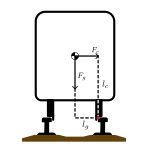
\includegraphics[width=0.33\textwidth]{fig/tåg_krafter.png}
    \caption{Kraftsituationen på en järnvägsvagn vid en vänstersväng där $F_g$ är tyngdkraften, $F_c$ är centrifugalkraften och $l_g$ respektive $l_c$ är deras momentarmar till rotationsaxeln A.}
    \label{fig:tåg_krafter_sväng}
\end{figure}

\subsection{Empirisk metod}
Ett 3d printad modelltåg i skala 1:40 (Modellerat efter en SIEMENS Vectron, men hjuprofil S1002 (CITAT)) med en vikt på \num{1.4} kg, en kamera som filmar i minst 240 FPS, ett stativ för att hålla kameran, rutat papper (vars rutor har sidlängd 1 cm) och 3D printade rälssegment i skala 1:40 (utefter UIC60 standard (citat)) med radier: 80, 40, 25, 12, \num{6.5}, \num{3.5}, 2, 1 (m). 

Undersökningen kommer ske genom att det först väljs en specifik cirkelradie. Därefter kommer tåget placeras en bestämd höjd upp på en kulle. Anledningen till detta är att formeln för tågets potentiella energi då kan användas för att preliminärt beräkna hastigheten (sätt in formler). Om tåget inte spårar ur vid denna hastighet kommer det placeras högre upp i kullen tills gränsen hittas. Då kommer inspelningen från kameran med hjälp av det rutade pappret användas för att mer exakt bestämma hastigheten, denna hastighet tillsammans med radien kommer sedan sparas och användas i resultaten. Detta repeteras sedan med de andra bestämda radierna. När maxhastigheter har hittats för alla radier kommer fördelningen av vikten i tåget förflyttas genom att vikter i tåget placeras högre eller lägre ned. 

När all data har samlats in kommer den användas för att skapa en regression med hastighet och radie som grafaxlar. Detta kommer göras separat för varje viktfördelning. 

\subsection{Tidsplan}
vecka 40:
göra klart Projektplans utkastet och beställa kullager samt axlar till tågmodellen

Vecka 41: senaste dagen att lämna in projektplanen (måndag kl 1200) samt renskrivning av projektplan och mer inläsning av fysikaliska och matematiska modeller. utöver detta kada klart tågmodellen

vecka 42: samma som tidigare

vecka 43: inlämning av slutlig Projektplan

Vecka 44: höstlov

vecka 45: slutliga förberedelser för labben och ihopsättning/ kontrollering av modellens kvalite

vecka 46: om modellen visar sig vara av sämre kvalite; bygg om modellen, annars påbörja labben

vecka 47: simulering av experiment på KTH om tiden funkar för båda grupper, annars fortsättning med experiment

vecka 48: analys av data

vecka 49: formulera resultat

vecka 50: workshop statistik med excel

vecka 51-1: lov

vecka 2: genomgång felanalys

vecka 3: fortsätt bearbeta resultat och börja med att skriva ned dem

vecka 4: skriva resultat och diskussion

vecka 5: genomgång av naturvetenskaplig rapport och börja skriva resultat och diskussion

vecka 6: fortsätt skriva och börja med abstrakt när vi blir klara med tidigare delar

vecka 7: fortsätt skriva

vecka 8: fortsätt skriva

vecka 9: lov/kris skrivning

vecka 10: genomgång av hur oppositionen går till samt skrivning

vecka 11: inlämning av raport inför oppositionen

vecka 12: förberedelse av oppositionen

vecka 13: oppositioner

vecka 14: oppositioner

vecka 15: lov

vecka 16: revidering av rapport

vecka 17: gymnasiearbetes dag med åk 2

vecka 18: slutinlämning av rapport och allt annat (slut)